\chapter{调制识别的深度框架研究}

\section{引言}

尽管机器学习的目的是提供一种通用的问题解决算法,但目前性能最优的网络模型大部分仍然是对应于特定应用的。
目前存在几种较完善的网络,比如包括多层感知机、RNN、CNN及其许多变体以等,
他们被应用在各个领域,取得了很好效果。
然而,由于模型所面对的环境不同,数据不同,数据分布也不同;
因此,其他领域的很多模型对于我们的调制识别任务并不一定完全适应,需要我们进行相应的探索。 \par

在第三章中,我们基于网络模型的层面,提出了一种不同类型深度模型融合的深度网络框架,
并将其应用到无线信号调制识别任务中,而且取得了一定的性能提升。
在本章中,我们将以LeCun的经典五层网络结构为基准,从网络底层研究网络超参数对调制识别性能的影响,
并从欠拟合与过拟合的角度来理解出现这些现象的原因。\par

\section{系统模型}

在大部分现有的深度神经网络中,卷积层是它们共有的基本网络单元。
每个卷积层由若干个卷积核组成,每个卷积核通常非常小(1x1到5x5是图像处理中的常见尺寸)。
在传统的DSP应用中,卷积核通常设计得非常宽,而非设计成很深的多层结构。
计算机视觉领域中,神经网络的一个明显趋势是建立更深的网络来学习更复杂的函数变换和层次特征关系。\par

标准卷积层【】的传递函数在方程\ref{eqt_5_1}中给出:
\begin{equation}
	\label{eqt_5_1}
	f(I_i) = f (b_j + \sum_{i}(k_{ij} * I_i))
\end{equation}

其中,$f(I_i)$是第$i$个卷积核的输出特征图(Featrue Map),
$b$和$k$表示卷积核的偏置和卷积核的权重参数,$I_i$代表卷积核的输入 值,$*$ 表示卷积运算,
并且$f(\dot)$表示诸如整流线性单元($ReLU$)或$Sigmoid$单元等激活函数。\par

本章中,我们所有的网络结构都是基于图\ref{fig_5_0}的框架,基准的卷积神经网络在$Softmax$分类层之前有两个卷积层和一个全连接层,Softmax层之后输出样本分类结果。\par
\begin{figure}[!htbp]
	\centering
	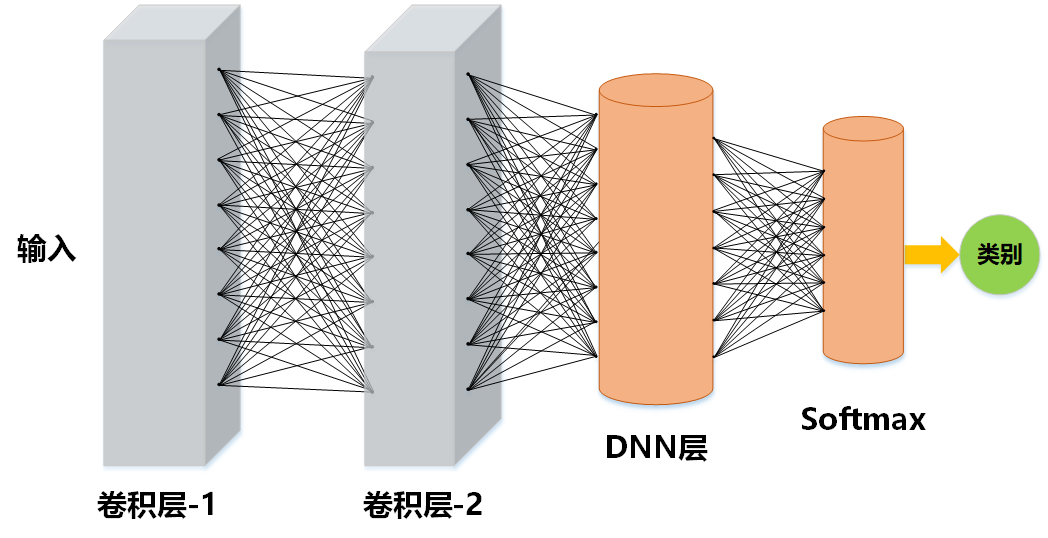
\includegraphics[scale=0.6]{figures/chapter_5/fig_5_0}
	\caption{本章所用CNN网络框架}
	\label{fig_5_0}
\end{figure}

整个网络中,我们所变化的只是网络的层数、卷积核的高度和宽度、卷积核的数目等这几个超参数。
我们所有的模型训练都将使用Adam优化器,因为它提供了梯度归一化和动量的方法,
降低了像学习率这样的超参数对模型训练结果的影响。
每个卷积层和隐藏层都使用整流线性单元(ReLU)作为激活函数,并使用$dropout=0.5$来降低模型的过拟合,
而预测时,我们使所有的单元处于激活状态。\par

\subsection{模型的偏差与方差}
\label{sec_5_2_1}
偏差恒量机器学习算法对于输入样本的期望输出与真实值的偏离程度,本质上表征了机器学习算法本身的拟合能力。
方差表示算法性能随训练集的变化而产生的波动,本质上表征了数据扰动所对算法性能的影响。
噪声则表示当前任务下,我们的训练数据与数据的真实值之间的差距,即任何学习算法所能达到的期望泛化误
差的F下界,衡量了学习任务本身的难度。\par

我们假设调制识别的训练样本集为$X$,$Y$为训练样本的真实类别。
对于训练集中的每一个样本$x_i \in X$,假设其真实类别为$\hat{y_i}$,$y_i$为在训练集中的类别。
在训练集$X$上学得模型$\phi(\dots)$,$\phi(x_i; X)$为输入样本为$x_i$时的输出,即预测类别:
\begin{equation}
	\label{eqt_5_2}
	y_i = \phi(x_i), x_i \in X
\end{equation}

我们假设网络预测的期望为:
\begin{equation}
	\label{eqt_5_3}
	\overline{\phi}(x) = E_X\left[ \phi(x; X) \right]
\end{equation}

如果我们使用相同数目的不同训练样本集$\hat{X}$进行训练,那么我们有方差:
\begin{equation}
	\label{eqt_5_4}
	\delta_{\hat{X}}^2(x) = E_{\hat{X}}\left[ (\phi(x, \hat{X}) - \overline{\phi}(x))^2\right]
\end{equation}

此时,模型的噪声为$\epsilon^2 = E_{\hat{X}}\left[ (\hat{y} - y)^2\right]$,
表示训练数据与真实数据的误差情况。
模型的期望输出与真实标记的差别为偏差,即:
\begin{equation}
	bias^2(x) = (\overline{\phi}(x)  - \hat{y})^2
\end{equation}

我们假设噪声期望为$0$,即$E_{\hat{X}}[\hat{y} - y] = 0$,由【】我们有泛化误差为偏差、方差与噪声之和:
\begin{equation}
	E(\phi; X) = bias^2(x) + \delta_{\hat{X}}^2(x) + \epsilon^2
\end{equation}

为了简化模型的分析,我们假设所有的训练样本都是无偏的,
即对于任意训练样本$(x_i, y_i) \in X$,我们有$\hat{y}_i \equiv y_i$。此时我们有泛化误差$E(\phi; X) $:
\begin{equation}
	E(\phi; X) = bias^2(x) + \delta_{\hat{X}}^2(x) 
\end{equation}

因此,我们可以从降低偏差和方差的角度出发,来提升模型的性能。

\subsection{过拟合与欠拟合}

在训练机器学习模型时,我们以降低训练误差为目标,获得模型的参数。
然而,我们不仅希望学习算法在训练集上表现良好,更希望其在非训练的数据集上同样具备良好的性能。
泛化正是衡量机器学习算法在未知数据上表现能力良好的一种定性标准。
泛化误差可以定义为模型对于新输入未知样本的误差期望。
欠拟合是指模型不能在训练集上获得足够低的误差,而过拟合是指测试误差大于训练误差。\par

模型的容量是指模型的拟合能力。
容量较低的模型其拟合能力较弱 ,很难反映训练集的数据分布。
容量高的模型,由于其拟合能力过强,可能会将噪声数据也学习到模型中,从而发生过拟合。
我们可以通过调整模型的容量,控制模型是否倾向于过拟合或者欠拟合。\par

通过小节\ref{sec_5_2_1}中的结果可知,
模型的泛化性能是由学习算法本身的拟合能力、数据的充分性以及学习任务本身的难度共同决定的。

对于给定的学习任务$T$,为了取得较好的泛化性能,我们需要使模型具备较小的偏差,即模型可以充分拟合训练数据,
并且还要使模型的方差处于较小值,即使得数据扰动对模型产生的影响尽量小。\par

然而,实际中偏差与方差却具备相反的倾向性。
在我们对算法进行训练时,
如果训练不足, 则机器学习模型的拟合能力不够强,训练数据的扰动不足以使模型产生显著变化
,此时偏差主导了泛化误差;
而随着训练程度的加深,模型的拟合能力逐渐增强,训练数据产生的扰动逐渐能被模型所学习,
此时方差逐渐主导了泛化误差;
在训练程度达到临界条件以后,如验证误差超过了训练误差一定阈值,模型的拟合能力已经非常强,
训练数据发生的轻微扰动都会导致模型发生显著的变化,
此时,模型可能学习到训练数据某些样本自身的、非全局性的特性,这就会产生模型的过拟合。\par

\section{网络超参数对调制识别的影响}
网络的超参数,如学习速率,每层卷积核的数量,卷积核的大小以及卷积层的数目等,
会影响网络规模,特征提取的数目等,如果不具备一定的领域先验知识很难优化。\par

在本节中,我们将研究网络卷积核以及卷积层等相关超参数对分类性能的影响,
这可以为我们后续的研究提供一定的网络整体架构的参考,节省了后续研究的时间成本,
并有助于进一步探究新的网络底层架构,以提升调制识别的性能。\par

\subsection{网络层数对调制识别的影响}

在本小节我们将探索网络层数对调制识别的影响。
由于我们仅仅是探索卷积层深度对分类性能的影响,而且网络的训练本身是一个非常耗时的过程。
因此,为了降低时间成本并简化分析提供一个定性的结果,我们在本小节中的仿真所有卷积核数目都为$32$,
并将卷积核的大小从$1\times3$到$1\times12$变化。\par
网络层次深度对训练数据遍历次数的要求差别很大,
为了解决这个问题,我们将所有的网络$epoch$设置为一个较大值(本文中$epoch=500$),
以满足那些对于复杂网络对于较高次数$epoch$训练的需求。
同时,我们使用了预停止策略,假设训练过程中,训练损失在$N_{pre\_stop}$(本文中我们设置为$N_{pre\_stop}=10$)个$epoch$内不降低,
即在这段训练时间范围内,模型不能得到很好的优化,此时我们则会停止训练。
这样便可以在尽量保证准确率的同时提高训练效率。\par

根据我们的预设条件,系统的仿真结果如图\ref{fig_5_1}所示。\par
\begin{figure}[!h]
	\centering
	\subfloat[3D展示]{
		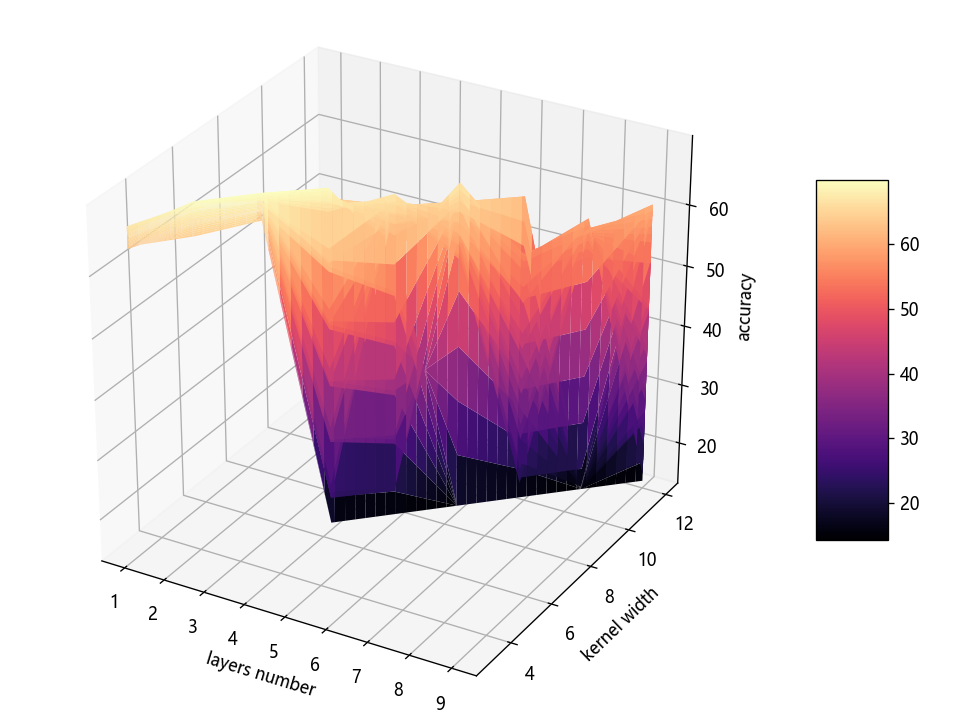
\includegraphics[width=0.5\linewidth, height=0.4\linewidth]{figures/chapter_5/fig_5_1}
		\label{fig_5_1_a}}
	\subfloat[热力图展示]{
		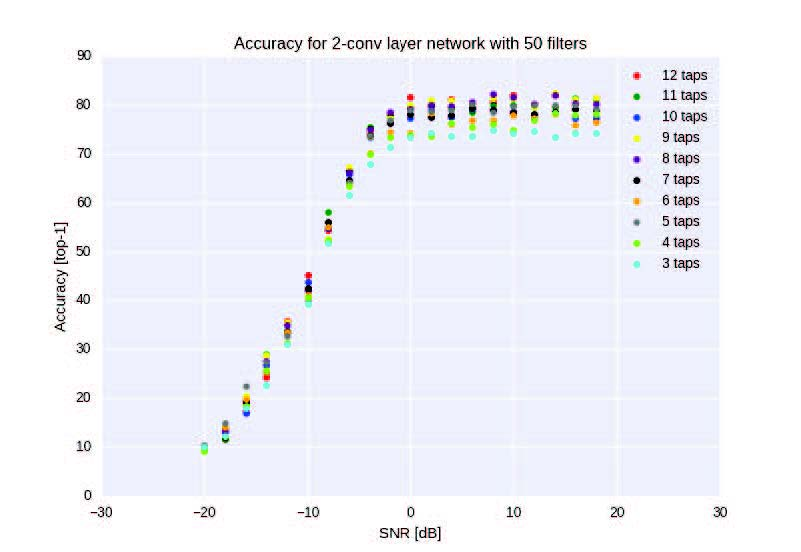
\includegraphics[width=0.5\linewidth, height=0.4\linewidth]{figures/chapter_5/fig_5_2}
		\label{fig_5_1_b}}
	\caption{不同卷积核宽度下,卷积层数目对分类准确率的影响}
	\label{fig_5_1}
\end{figure}

通过图\ref{fig_5_1}我们可以发现,分类性能具有一个相对整体性的趋势:
当卷积层大于3时,分类准确率几乎成下降趋势。
通过图\ref{fig_5_1_a}我们可以发现,系统性能在卷积层为$3$,卷积核的宽度为$6$以上时,
系统性能能够达到一个较高的水准;同时我们可以发现卷积核宽度较大时,
卷积核层数在大于$3$时分类准确率几乎呈一个断崖式下跌。\par

在图\ref{fig_5_1_b}中我们可以清楚地发现,整幅图像在卷积层数目较大、卷积核数目较小时,系统的性能较差。
卷积层数目小于$4$时,系统性能随卷积核宽度变化不大,增大卷积核宽度并不能很大程度上提升系统分类性能;
卷积层较大时,增加卷积层的宽度反而会降低系统性能。\par

接下来,我们以卷积层数目作为变量,观察不同卷积核宽度条件下的分类性能,结果如图\ref{fig_5_2}。
\begin{figure}[!h]
	\centering
	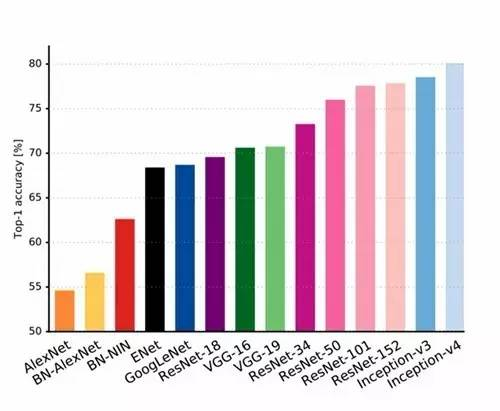
\includegraphics[scale=0.6]{figures/chapter_5/fig_5_4}
	\caption{分类准确率随卷积层数目和卷积核宽度的变化}
	\label{fig_5_2}
\end{figure}

从图\ref{fig_5_3}可以发现,整体而言,不同卷积核宽度的平均分类准确率,随着卷积层数目增加,
首先先轻微地上升,然后出现较大幅度的下降。\par

增加卷积层的深度,在卷积层数目$N_{layers} \leq 3$时,可以微小地改善分类性能。
当卷积层深度$N_{layers} \geq 4$时,改变卷积层的数量在分类准确率几乎都呈下降趋势;
但是,不同卷积核宽度的网络性能下降程度不同,
卷积核宽度较大的网络越,随着卷积层深度的增大性能下降程度较低。
在卷积层深度$N_{layers} \leq 3$时,我们发现分类性能几乎随着卷积核宽度的增加而增加,
直到卷积核宽度达到$11$时,达到分类性能的上限;
同时,我们发现分类性能在此时随着卷积层数增加而增加。\par

在卷积层数较低时,分类性能有所增加,
这可能是因为模型的拟合能力不足以完全表征信号的特性。
在卷积层数$N_{layers} \geq 4$时,网络性能大幅下降;
因为卷积核宽度较大时,分类性能仍然处于一个较高的水准,而且分类性能会随着卷积层数目的增加而发生剧烈的突变,
所以我们可以确定此时导致分类性能下降的主要原因是网络的训练难度增加;
其次,网络性能在卷积层数目为$3$时达到了性能的最高点,之后性能一直呈下降趋势,
我们认为这是网络发生过拟合的一个节点。
这表明对于我们的数据而言,可能是由于调制数据通常只改变正弦曲线的幅度,频率或相位,
因此对于调制方式而言数据的复杂度并不高,没有必要学习更高层次的深度特征。
\par

%然而,令我们意外的是,添加更多的卷积层似乎并不能在低信噪比下提高分类器的性能。
%这可能是由于在低信噪比下,由于噪声能量占比过高,覆盖了调制数据本身的特性,
%而深度网络更多的是对加噪之后的数据的数值特性进行特征提取,对于统计量、循环谱等特性并没有涉及,
%因此低信噪比下分类器的识别性能并没有得到提高。\par
%
%尽管添加更多卷积层不会提高分类准确性并不奇怪,但出乎意料的是分类和损失在3个卷积层之后快速提高。
%最初的研究结果表明,较深的网络会导致较高的训练损失。


\subsection{卷积核数目对调制识别的影响}
上一小节我们探究卷积层数目对调制识别的影响,本节我们将对网络结构进行更细化的研究,
探索卷积核数目对调制识别的影响。\par

通过在第三章的探索,我们发现卷积层在第一个卷积层为$1x5$的卷积核大小,第二个卷积层为$2x6$的大小时,有较好的分类性能。
因此,在本小节中,我们继续使用这样的卷积核维度,进行卷积核数目对分类性能影响的探索。\par
由于我们训练神经网络时间成本较高,很难对每一个卷积核数目参数进行遍历,所以我们选择一些有代表性的参数进行试验,主要目的是定性的分析卷积核数目的变化对于分类性能的影响。本论文中我们定义卷积核数目集合$\kappa =\{24, 32, 48, 64, 80, 96, 128, 160, 192\}$,
第一个卷积层与第二个卷积层分别从集合$\kappa$中选取,每层卷积核数目从$24$变化到$193$。
这样两个卷积层的核数目组合共有$|\kappa|^2$种,即网络训练总的遍历次数为$|\kappa|^2$。\par
通过仿真,我们最终得到分类器性能随卷积核数目变化的结果如图\ref{fig_5_1}所示:\par
\begin{figure}[!h]
	\centering
	\subfloat[3D展示]{
		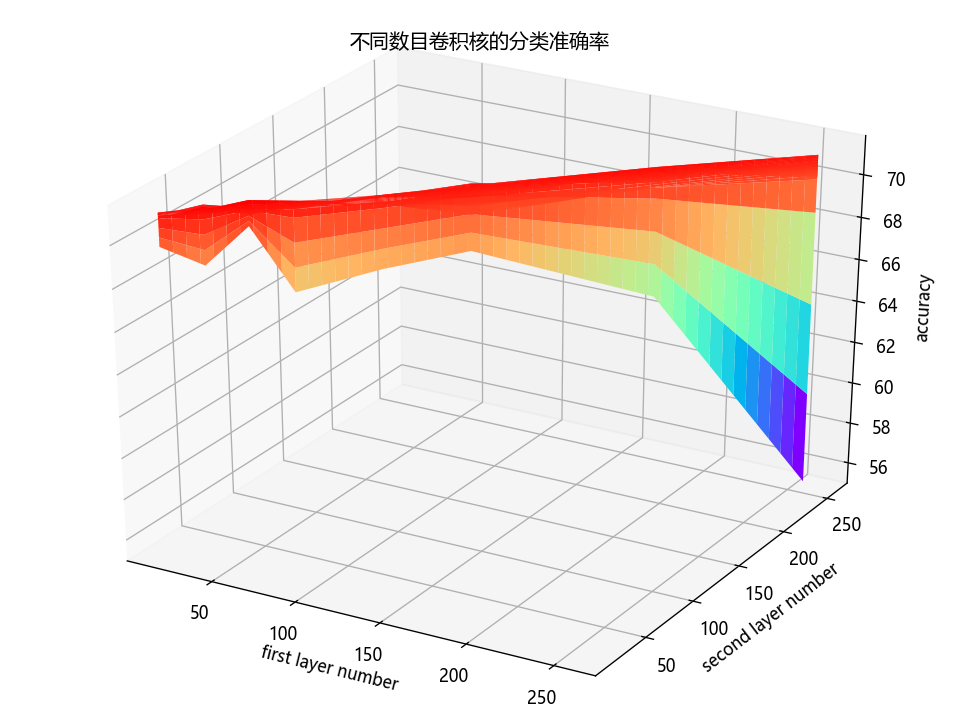
\includegraphics[width=0.5\linewidth, height=0.4\linewidth]{figures/chapter_5/fig_5_9}
		\label{fig_5_3_a}}
	\subfloat[热力图展示]{
		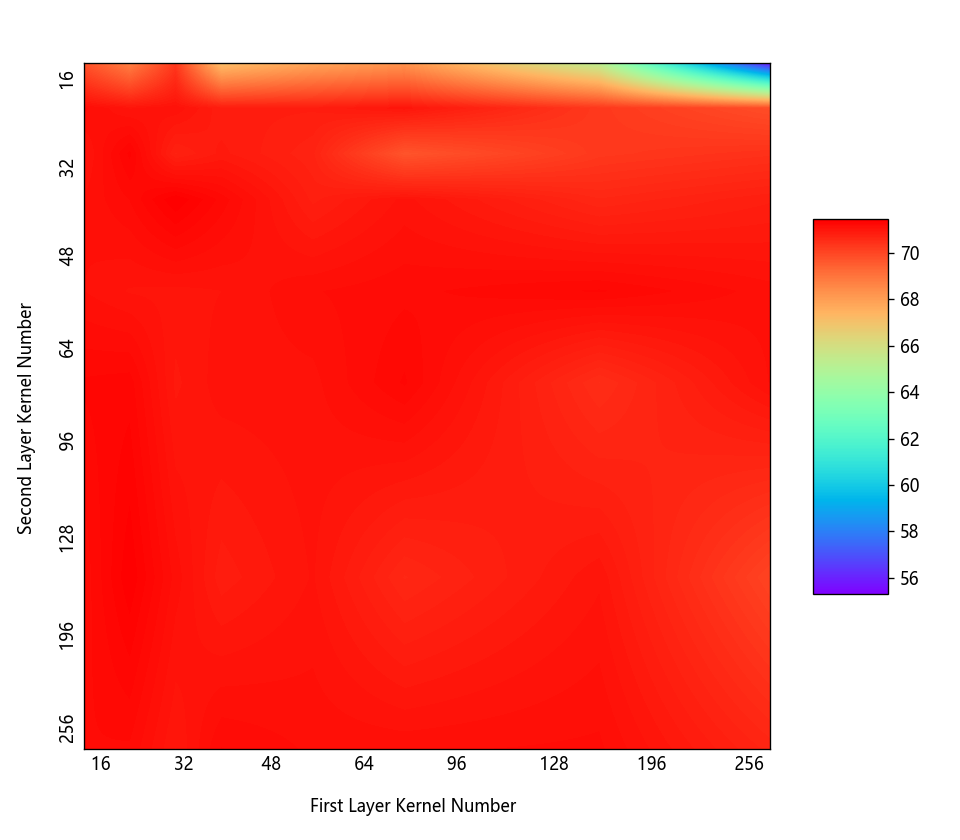
\includegraphics[width=0.5\linewidth, height=0.4\linewidth]{figures/chapter_5/fig_5_10}
		\label{fig_5_3_b}}
	\caption{卷积核数目对分类准确率的影响}
	\label{fig_5_3}
\end{figure}

\begin{figure}[!h]
	\centering
	\subfloat[3D展示]{
		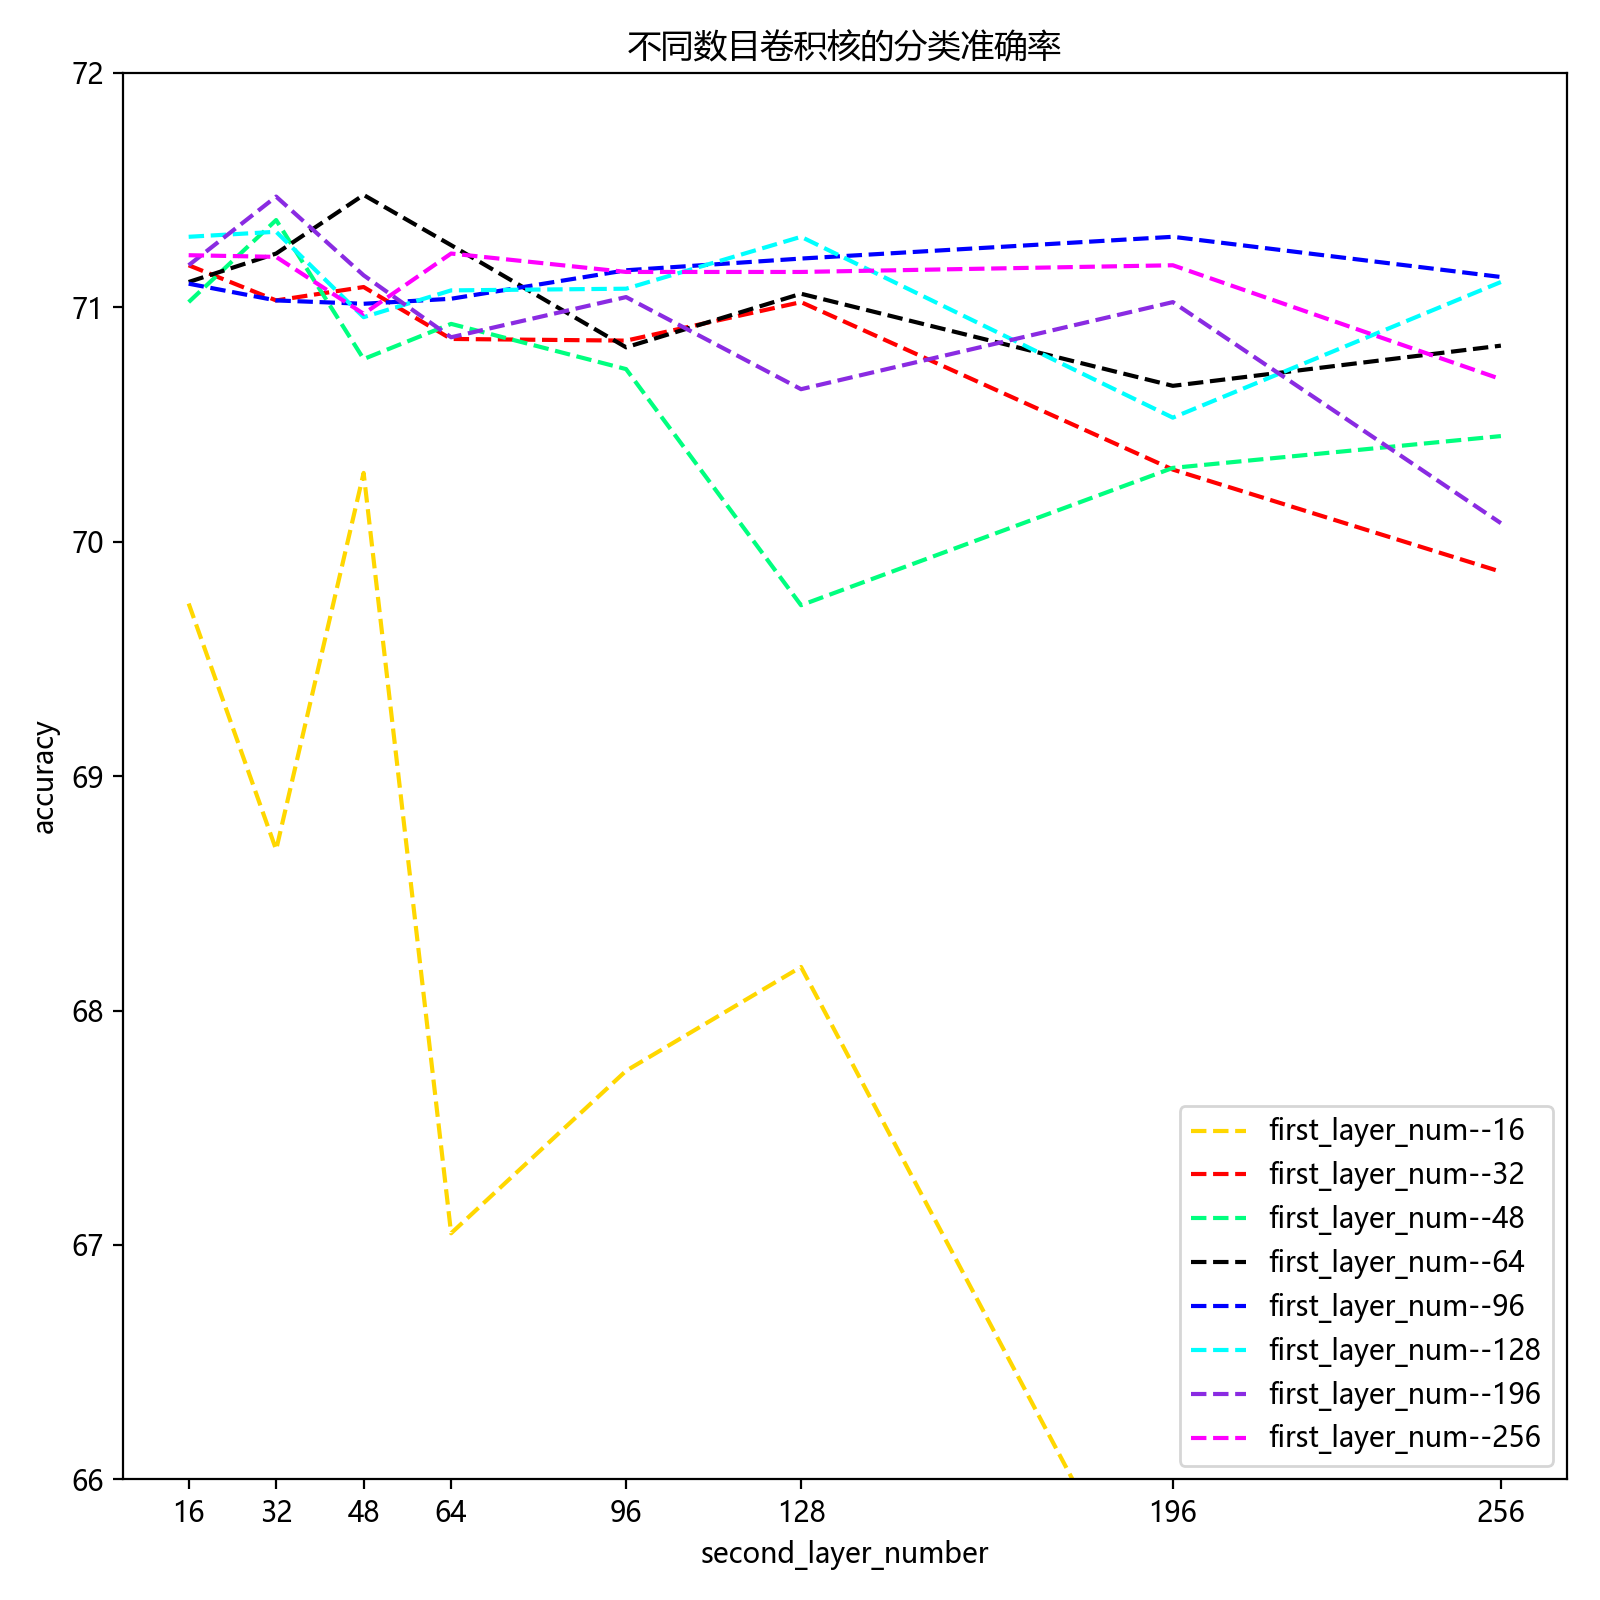
\includegraphics[width=0.5\linewidth, height=0.4\linewidth]{figures/chapter_5/fig_5_11}
		\label{fig_5_4_a}}
	\subfloat[热力图展示]{
		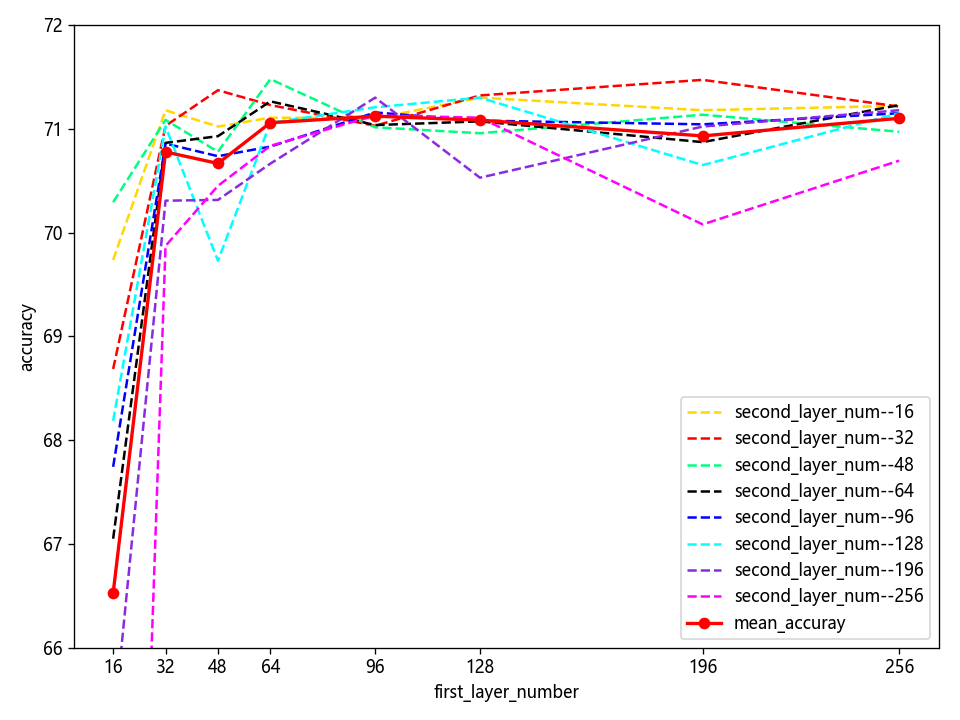
\includegraphics[width=0.5\linewidth, height=0.4\linewidth]{figures/chapter_5/fig_5_12}
		\label{fig_5_4_b}}
	\caption{卷积核数目对分类准确率的影响}
	\label{fig_5_4}
\end{figure}

\begin{figure}[!h]
	\centering
	\subfloat[3D展示]{
		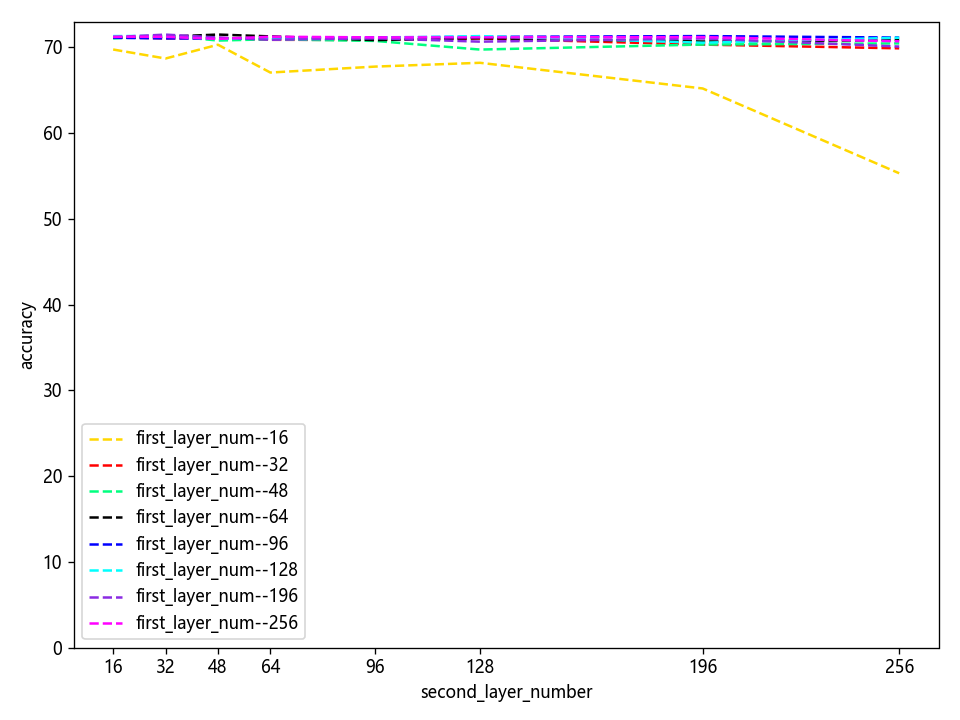
\includegraphics[width=0.5\linewidth, height=0.4\linewidth]{figures/chapter_5/fig_5_13}
		\label{fig_5_5_a}}
	\subfloat[热力图展示]{
		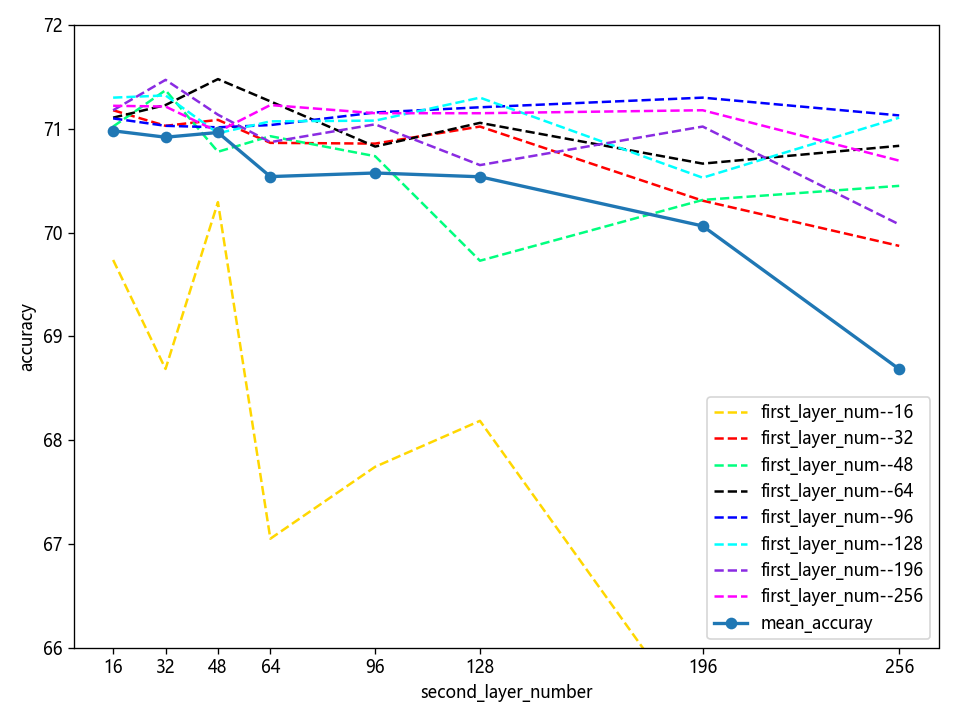
\includegraphics[width=0.5\linewidth, height=0.4\linewidth]{figures/chapter_5/fig_5_14}
		\label{fig_5_5_b}}
	\caption{卷积核数目对分类准确率的影响}
	\label{fig_5_5}
\end{figure}


图\ref{fig_5_1}显示了卷积核数量从24增加到90时,信噪比为0dB时的$7$类信号分类准确率。通过图\ref{fig_5_1}的结果我们可以发现,当第一层和第二层的卷积核数量较小时,分类的准确率处于一个比较低的水准;当第一层和第二层的卷积核数目增加时,分类准确率相应的增加;当第二个卷积层数目增加到64时,网络的分类性能不再随着第一层卷积核数目增加而增加;当第二个卷积层中卷积核的数目大于64时,不管第一层卷积核数目如何变化,分类性能都不能超过最值。通过综合考虑两个卷积层,我们可以发现当第一层卷积核数目为64、第二层卷积核数目为32时,分类器性能达到最优。\par
对于这种现象出现的原因,通过分析,我们认为卷积核数目从网络的复杂度以及网络的特征提取维度两方面影响分类的性能。\par
当卷积核数目很小时,同时由于网络本身的深度较小,因此,受限于卷积特征图数目的限制,特征提取的数目也相应的较少,很难较完整地反映数据本身的特征,分类准确率的上限会出于一个较低值。当卷积核数目增加,相当于我们的特征数目也在相应的增加,这样,网络本身的拟合能力增强,卷积核所提取的卷积特征能更好地反映数据的内在特征,因此,分类性能的上界相应提高,可以获得较好的分类结果。\par
当卷积核的数目增大到一定的程度,网络的拟合能力过强,不仅能够拟合出数据本身的性质,同时将一些异常点也进行了拟合,这就造成了过拟合;同时,由于我们的数据量有限,也很难将网络参数训练到一个较优的水平。因此,我们的分类性能可能会随着卷积核数目的增加而降低。\par

\subsection{卷积核大小对调制识别的影响}
在本小节我们将探究卷积核大小对调制识别性能的影响。根据第三章我们采用的卷积神经网络结构,我们将第一个卷积层的卷积核数目固定在64,将第二个卷积层的卷积核数目固定在32,因为这种情况下网络具有较好的分类性能。\par
我们假设卷积核高度在$0$与$1$之间变化,卷积核的宽度在$3$到$9$之间变化。则总的训练迭代次数为$7 * 7 * 2 * 2$。为了弱化不同网络结构对训练样本$epoch$次数的需求,我们假设$epoch=1000$,这是一个很大的值,但是我们自定义了预停止策略:当每次训练迭代时,$epoch$次数增大10次,而分类性能没有提升,我们则停止本次的训练迭代。整个仿真在我们的硬件平台下大约持续了150小时,结果如图\ref{fig_5_2}所示:\par
\begin{figure}[!h]
	\centering
	\subfloat[3D展示]{
		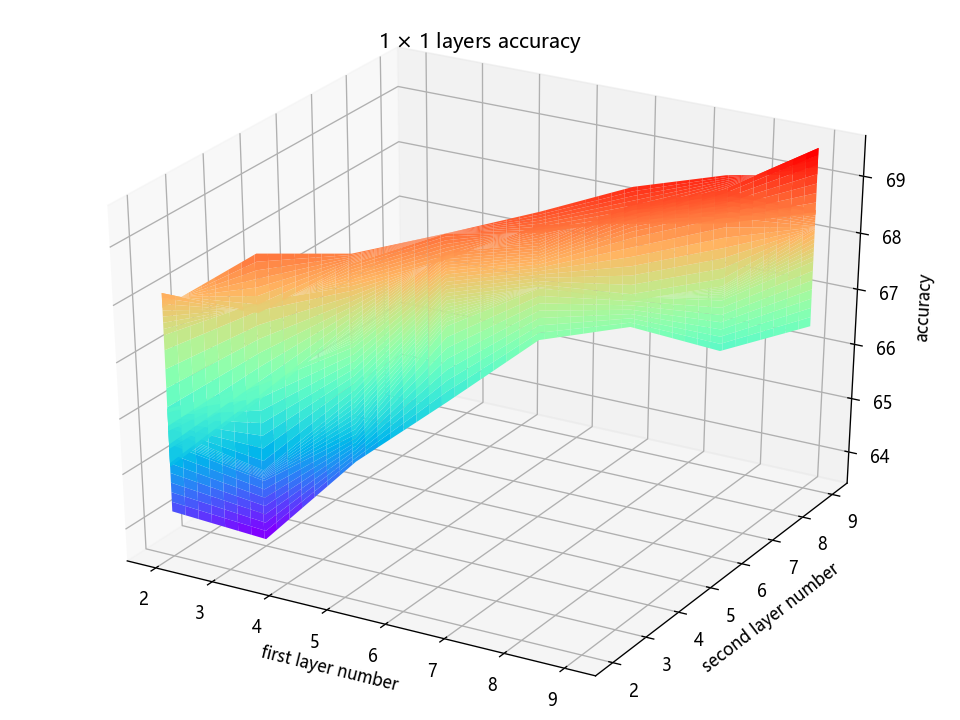
\includegraphics[width=0.5\linewidth, height=0.4\linewidth]{figures/chapter_5/fig_5_15}
		\label{fig_5_6_a}}
	\subfloat[热力图展示]{
		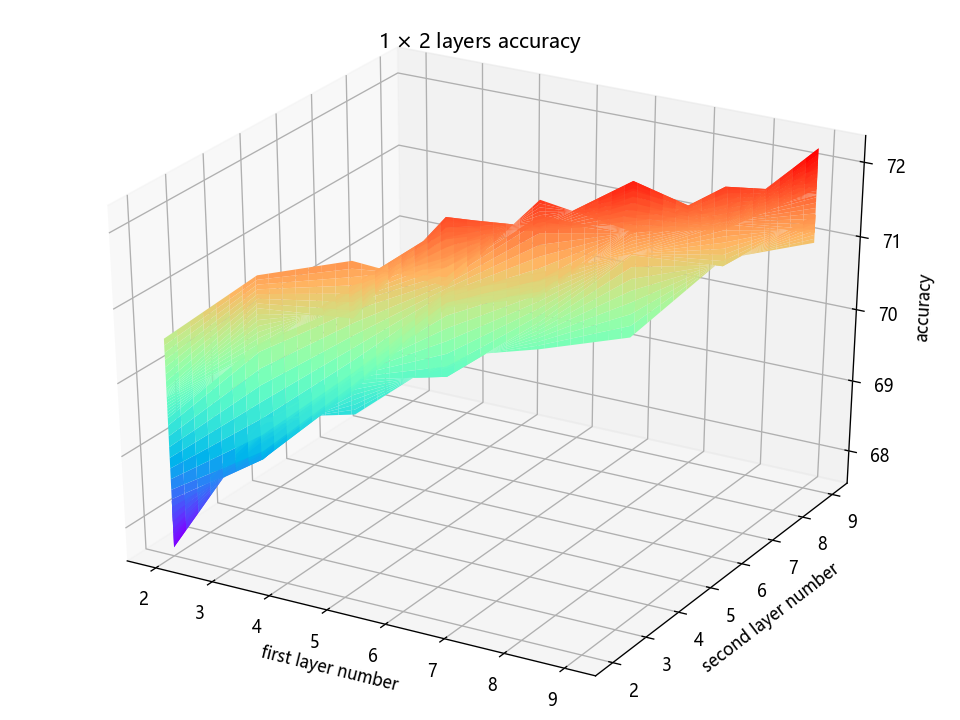
\includegraphics[width=0.5\linewidth, height=0.4\linewidth]{figures/chapter_5/fig_5_16}
		\label{fig_5_6_b}}
	\\
	\subfloat[3D展示]{
		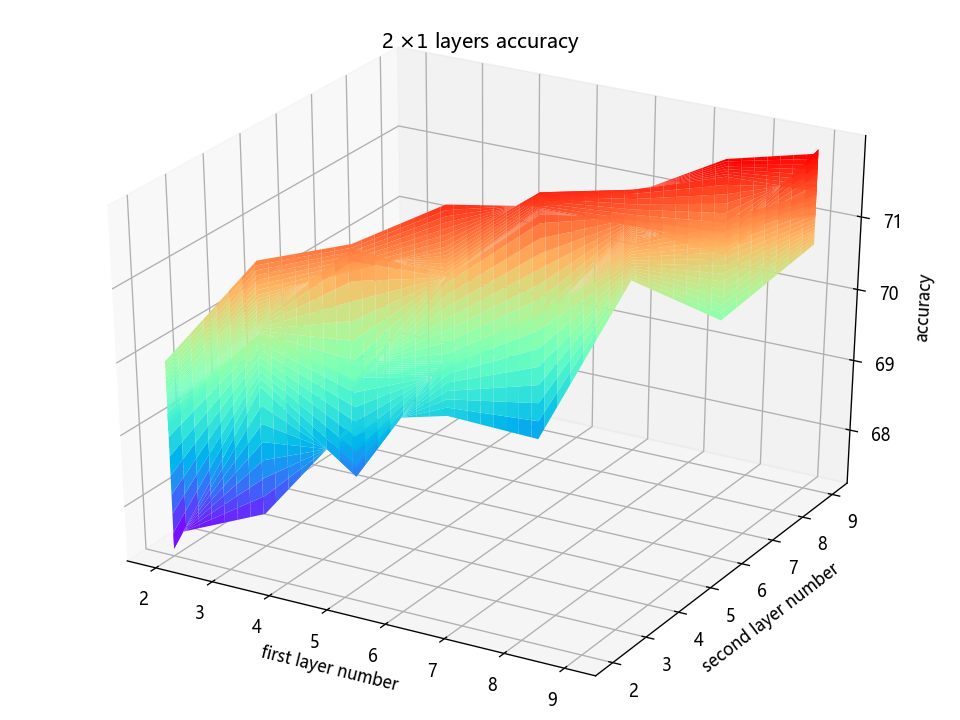
\includegraphics[width=0.5\linewidth, height=0.4\linewidth]{figures/chapter_5/fig_5_17}
		\label{fig_5_6_c}}
	\subfloat[热力图展示]{
		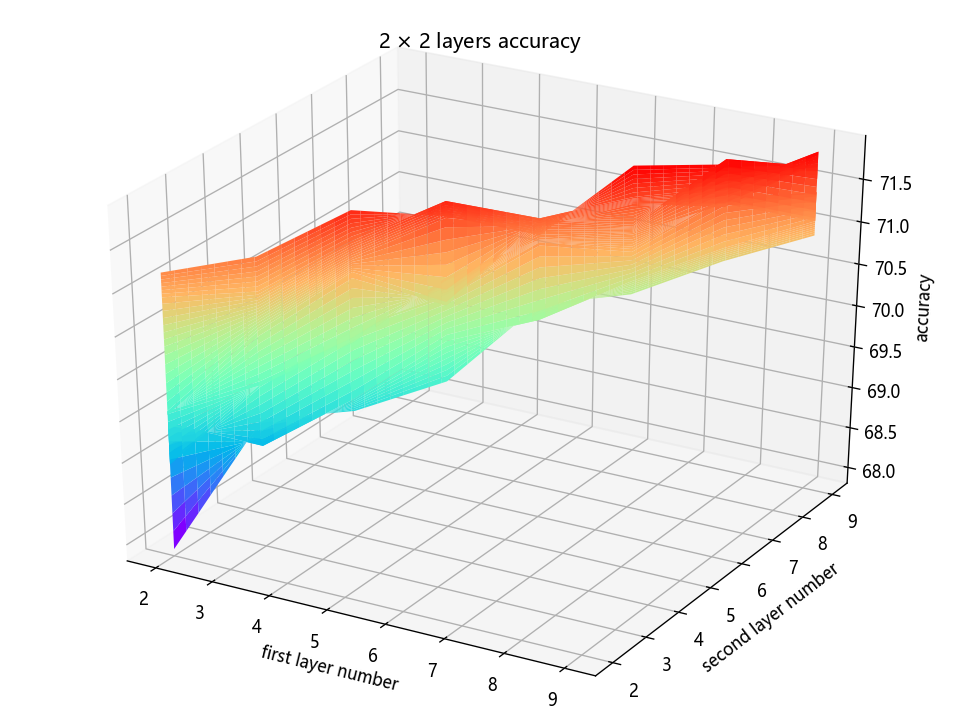
\includegraphics[width=0.5\linewidth, height=0.4\linewidth]{figures/chapter_5/fig_5_18}
		\label{fig_5_6_d}}
	\caption{不同卷积核宽度下,卷积层数目对分类准确率的影响}
	\label{fig_5_6}
\end{figure}


\begin{figure}[!h]
	\centering
	\subfloat[3D展示]{
		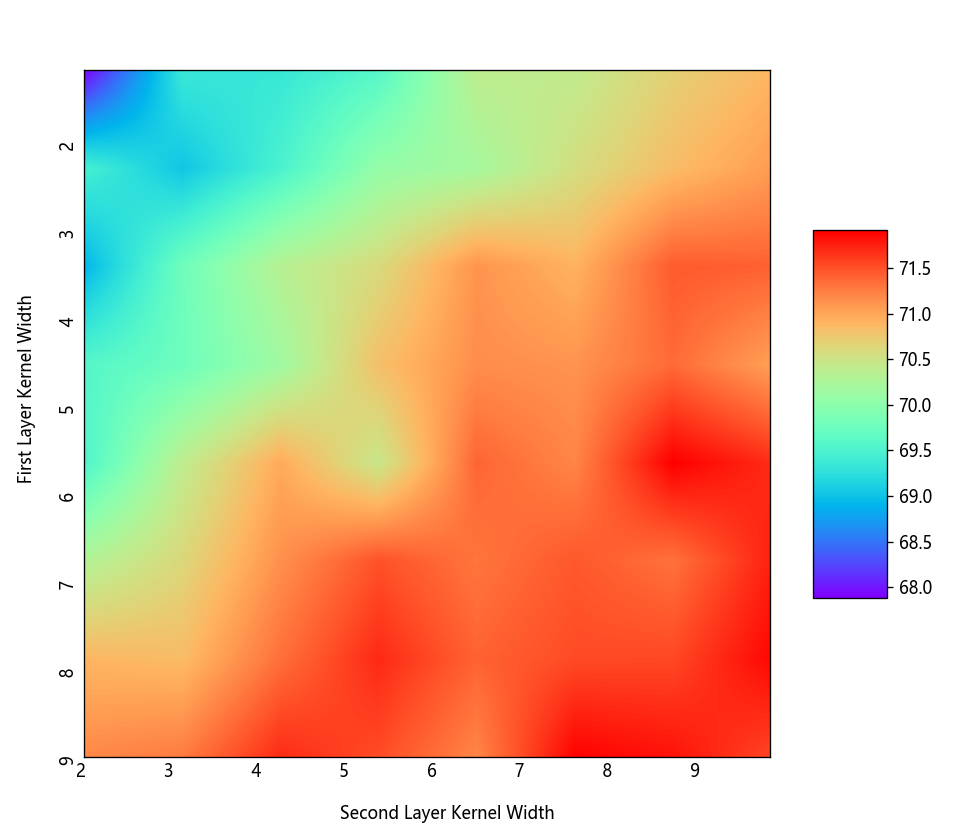
\includegraphics[width=0.5\linewidth, height=0.4\linewidth]{figures/chapter_5/fig_5_23}
		\label{fig_5_7_a}}
	\subfloat[热力图展示]{
		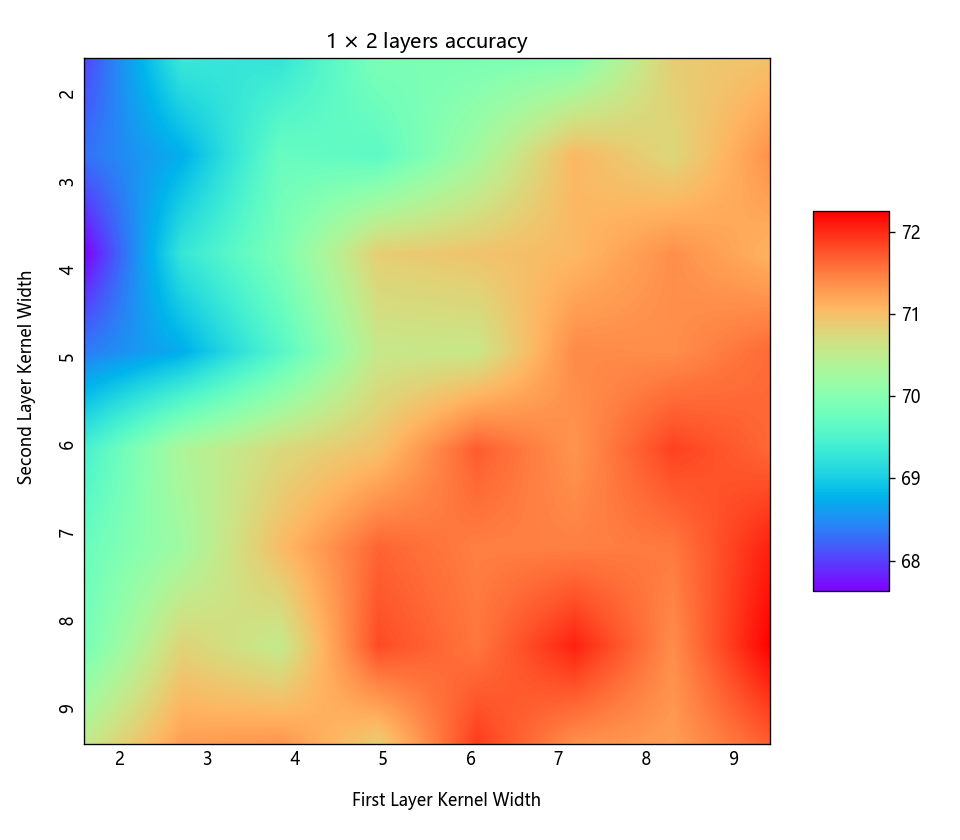
\includegraphics[width=0.5\linewidth, height=0.4\linewidth]{figures/chapter_5/fig_5_24}
		\label{fig_5_7_b}}
	\\
	\subfloat[3D展示]{
		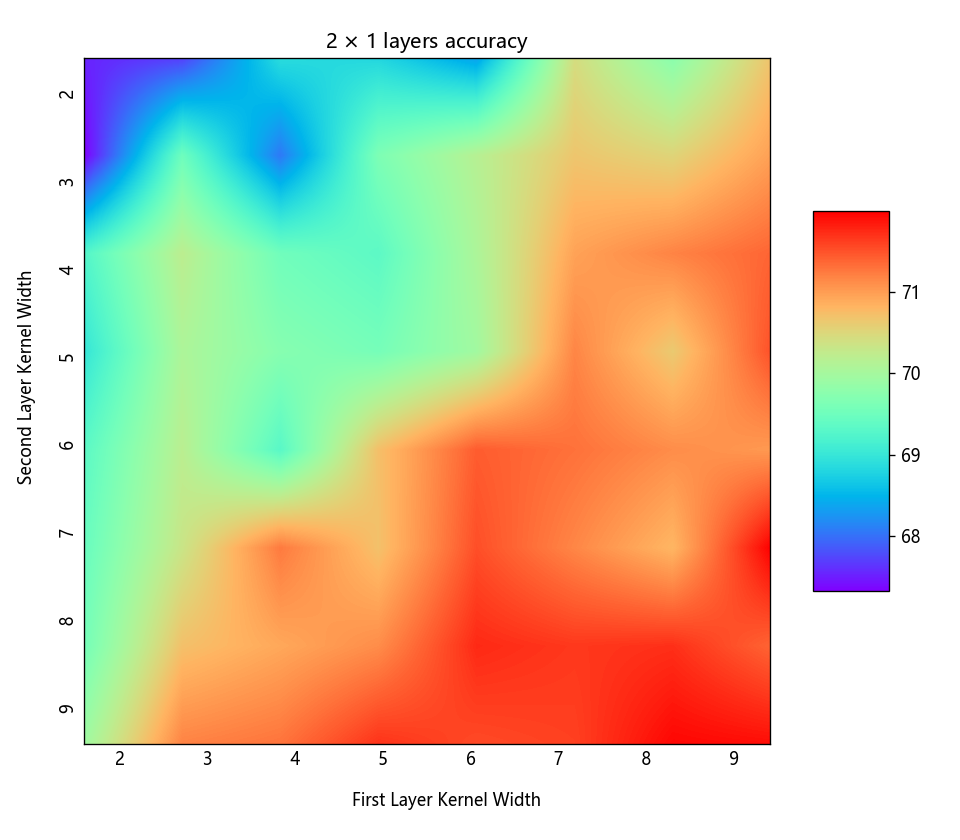
\includegraphics[width=0.5\linewidth, height=0.4\linewidth]{figures/chapter_5/fig_5_25}
		\label{fig_5_7_c}}
	\subfloat[热力图展示]{
		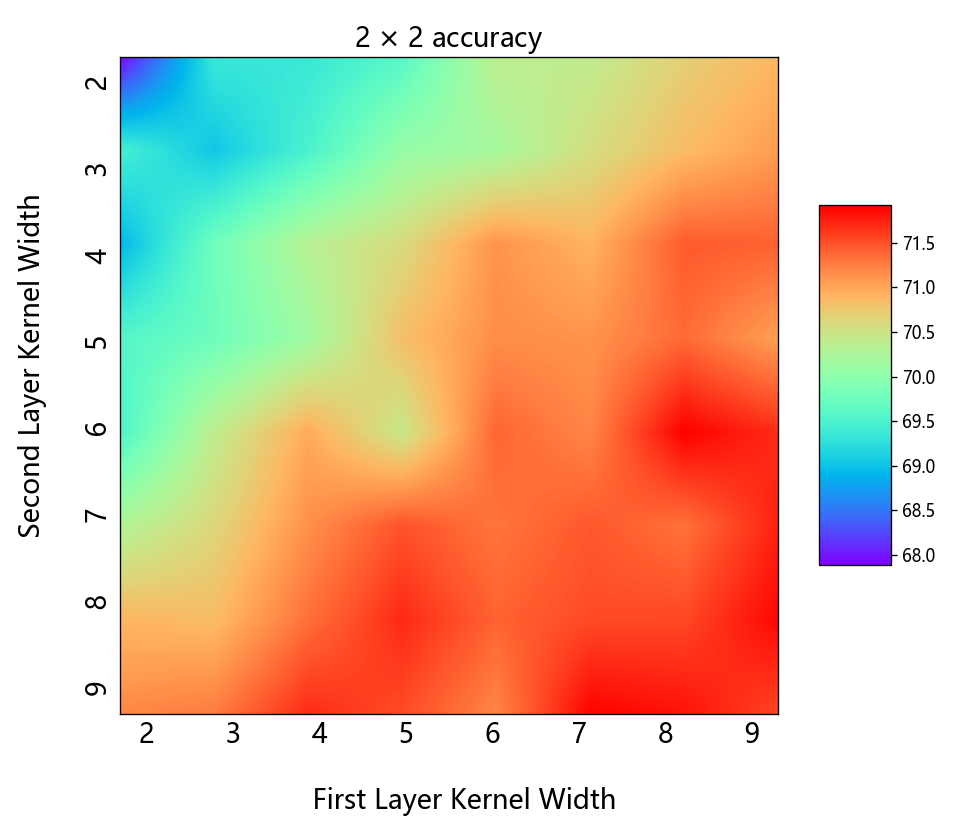
\includegraphics[width=0.5\linewidth, height=0.4\linewidth]{figures/chapter_5/fig_5_26}
		\label{fig_5_7_d}}
	\caption{不同卷积核宽度下,卷积层数目对分类准确率的影响}
	\label{fig_5_7}
\end{figure}

每个卷积层的卷积核尺寸变化的结果表明:1. 对卷积核的宽度而言,整体而言较小的卷积核不如较大的卷积核,但是当卷积的宽度增大到7之后,
分类性能变化很小;2. 对卷积核的高度而言,当第一层卷积核的高度为1,第二层卷积核的高度为2时,我们可以获得相对最优分类性能。\par

通过图\ref{fig_5_2}我们可以发现卷积核宽度为$6-9$时网络的分类性能可以达到一个较高的水准。
这些数目的卷积核宽度相互之间有一定的差异,但是考虑到网络能达到的只是一个局部极小值,
而非全局极小值,我们很难定量的确定到底怎样的卷积核大小是一个最优值。
但是可以确定的是,由于我们的信号样本是128个采样点,而每个样本包含8到16个符号,也就是每个符号占用为$16$或者$8$个采样点。
因此,我们的卷积核宽度为$8$时,每次卷积操作相当于对$1$个符号或$1/2$个符号进行运算,
此时,分类器的性能很有可能达到一个相对较优的水平。\par

对于卷积层的高度而言,由于我们的样本是一个$2\times128$的时间序列,我们可以看成是由两行$128$维的向量组成。
其中,第一行表示信号的实部,第二行为信号的虚部。
这样,我们在利用卷积核对信号进行卷积特征提取时,如果卷积核的宽度为$1$,相当于是在信号的实部进行采样值的卷积运算;
如果卷积核的宽度为$2$表示我本不仅对信号进行实部的运算,同时考虑到了信号的虚部,
这样进行卷积时,可能同时会包含信号的能量信息。
当然,这些只是我们从理论层面的一些分析,具体卷积核维度变化相应于我们信号的哪一些特征,有待后续的进一步研究。
但是,可以确定的是,卷积的操作提取的不仅仅是某些确定的特征,
而很有可能是某些信号特性本身的体现,而且这些卷积特征随着参数的初始化、卷积核的维度变化所表征的含义也是完全不同的。\par

%\section{常见的网络架构}
%LeNet主要是用于识别10个手写数字的,但其具有较简单的网络底层结构,对于复杂数据识别效果较差。
%自2012年ImageNet竞赛之后,深度学习在之后大放异彩,表\ref{sec:table_5_1}是近几年主流的深度框架(AlexNet、VGG、GoogLeNet、ResNet)的比较。\par
%\begin{table}[H]\label{sec:table_5_1}
%	\centering
%	\caption{ ILSVRC历年Top-5错误率}
%	\begin{tabular}{ccccc}
%		\toprule
%		模型 & AlexNet & VGG & GoogLeNet & ResNet\\
%		\midrule
%		发布时间 &	2012 & 2014 & 2014 & 2015\\
%		\midrule
%		层数 & 8 & 19 & 22 & 152\\
%		\midrule
%		Top-5错误率 & 16.4\% & 7.3\% & 6.7\% & 3.57\%\\
%		\bottomrule 
%	\end{tabular}
%\end{table}
%AlexNet相比传统的CNN的改进主要在数据增强、dropout、池化、ReLU函数等,相较于我们提出的CNN基础框架没有本质上的区别。
%而VGG主要的改进是网络深度的改进,对我们的调制数据而言,网络深度的增加并不能带来模型性能的提升。
%因此,本文中我们对其影响并不作研究,而是主要对几个主流框架GoogLeNet、ResNet、CLDNN的底层结构进行改动适应调制信号的维度,
%并降低网络深度,观察不同的底层网络结构对调制识别的影响。
%
%\subsection{InceptionNet}
%GoogLeNet相较于CNN主要的创新在于提出了Inception结构,这是一种底层的网络结构,其类似于卷积核一样,是一种网络组成的单元。
%它可以提高网络深度和宽度,并能够将不同规模的特性推广到一般管理复杂性。
%Inception一直在不断发展,目前已经发展到$v4$版本,对于我们的调制识别应用场景,
%经过修改后基本的网络结构如图\ref{fig_5_4}所示:\par
%\begin{figure}[!h]
%	\centering
%	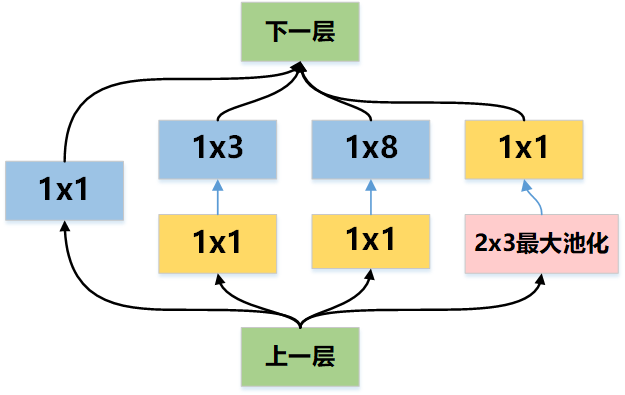
\includegraphics[scale=0.8]{figures/chapter_5/fig_5_27}
%	\caption{InceptionModel}\label{fig_5_27}
%\end{figure}
%每个Inception模块(如图\ref{fig_5_4}所示)包含四条并行路径,输出是四个并行输出的串联,
%用了Inception结构之后整个网络结构的宽度和深度都可扩大。
%第一条路径是一组对选定信息转发的$1\times1$卷积核,它只是简单地向前传递信息而不进行变换,
%可以使选择性信息高速前向传播。
%第二和第三条通道首先是$1\times1$卷积,接着是一组$1\times3$和$1\times8$卷积以提供多个宽度的特征检测。
%最后一条并行通道,首先是一个3x3池化层,接着是1x1卷积。\par
%我们在特征提取层中使用了两层适应性重构后的Inception网络,其中第一层包含32个Inception结构,第二层包含16个Inception结构。
%这样,我们可以保证在尽量不提高网络深度和宽度的情况下,学习数据的不同维度特征。\par
%
%\subsection{残差网络}
%残差网络(ResNet)的提出本质上是要解决层次比较深的时候无法训练的问题。
%使用跨层转发信息的体系结构是一种增加网络深度的有效方法,
%微软凭借ResNet的网络结构增加网络层深度至152层并赢得ImageNet 2015的冠军[4]。
%这种借鉴了Highway Network思想的网络相当于在主干网络之外开通一个特殊通道使得输入可以直达输出。
%图\ref{fig_5_5}展示了ResNet的基本结构:\par
%\begin{figure}[!h]
%	\centering
%	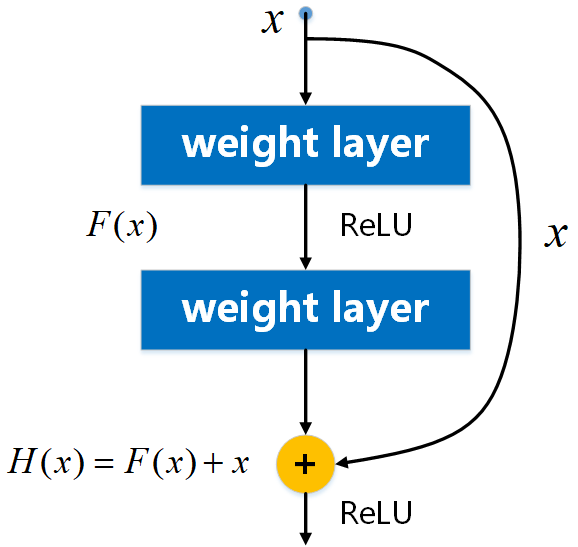
\includegraphics[scale=0.6]{figures/chapter_5/fig_5_28}
%	\caption{残差网络结构}\label{fig_5_28}
%\end{figure}
%如图\ref{fig_5_5}所示,,$x$是网络的输入,主干网络为输入信号$x$经过不同的网络层后向传播;
%同时,ResNet也会将一层的输出添加到更深层的两层输出中。
%其中$H(X)$是某一层原始的的期望映射输出,而优化的目标由原来的拟合输出$H(x)$变成输出和输入的差$H(x)-x$,
%由于ResNet的信息转发迫使网络学习残差函数进而学习数据的特征,因此这样的网络结构被称之为残差网络。\par
%ResNet的作者认为消失梯度可以通过广泛采用的归一化技术来解决,而深度网络的深度则受限于深度网络的训练复杂度,
%而残差网络正可以通过额外的信息转发通道,弱化网络深度对训练复杂度的影响。\par66
%
%由本章第二小节得到的结论,网络的深度并不是我们调制性能限制的主要因素。
%因此,我们在ResNet调制识别网络的设计时,仅仅考虑到使用五个层的简单网络,每隔两层进行信息转发,
%来探索ResNet的网络结构是否能提高调制识别的准确率。
%
%
%\subsection{卷积长短期深度神经网络}
%CNN可以减小频率的偏移变化,LSTM则很适合对时序语音进行建模,DNN就可以对特征进行非线性映射到一个抽象空间进行有效分离。
%卷积长短期深度神经网络(Convolutional Long short-term Deep Neural Networks,CLDNN)正是一种将CNN、LSTM和DNN结合的用于语音处理的算法。它在CNN上加入了对输入特征的时域卷积,同时实现了时域和频域卷积,并将时频域上的特征进行关联。\par
%
%受通信领域专业知识引导和CLDNN等网络体系结构的启发,我们最朴素的想法是采用典型通信接收器的通用结构,
%并构建具有类似结构的神经网络。
%通信接收机有一个卷积核(通常与传输的脉冲或波形匹配),同步器和采样器。
%通常,前置卷积核抽取每个符号的少量采样,用于执行相移以找到最佳采样点的同步器。
%与此类似的神经网络体系结构是卷积层,因此我们首先引入卷积层。
%LSTM广泛用于时间序列应用,由于我们是对时间序列信号进行分析获取调制方式,
%需要对时间特征进行建模,因此我们引入了LSTM单元组成的层。
% \par
%本论文中使用的CLDNN结构如图\ref{fig_5_29}所示:\par
%\begin{figure}[!h]
%	\centering
%	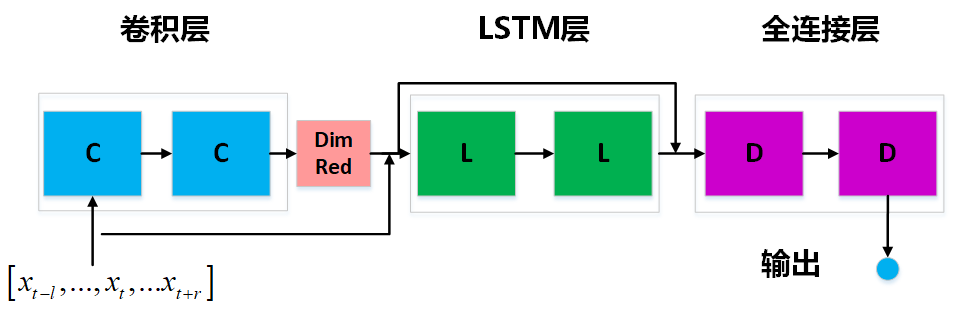
\includegraphics[scale=0.6]{figures/chapter_5/fig_5_29}
%	\caption{CLDNN结构}\label{fig_5_29}
%\end{figure}
%我们测试了两层和三层卷积的CLDNN型结构,其功能类似于卷积匹配卷积核。
%而在,由于数据本身不具备较高的复杂度,我们采用了两层的版本,实际证明两个卷积层的网络性能相对更优。
%随后是两个由长期短期记忆(LSTM)单元组成的循环层,其主要用于建模数据的时间特征。
%由于调制基带数据是时间序列,因此我们认为这对于整体的网络来说可能是一个较优的改进。
%CLDNN也可以具有绕过层的连接,旨在为数据提供更长的时间上下文信息。
%例如,原始CLDNN在LSTM层之前转发卷积层输出的原始样本到DNN层,此连接是原始波形和卷积输出的连接。
%我们尝试过有和没有前向连接,发现加入连接之后,网络的分类精度更高,梯度下降更稳定。\par
%
\section{结果及分析}

本节中,我们继续使用第三章中的数据集作为评估调制识别性能的基础。
我们使用所有信噪比条件下的$top-1$分类精率作为单个数字基准,并且比较信噪比在0dB时的分类精度。
所有模型的训练都基于Tensorflow深度学习库,平台系统配置如表\ref{sec:table_3_1}所示。\par

%
%\subsection{GoogLeNet分类混淆矩阵}
%
%\subsection{ResNet分类混淆矩阵}
%
%\subsection{CLDNN分类混淆矩阵}
%
%为了进一步理解什么限制了分类的准确性,我们看一下图1所示的CLDNN的混淆矩阵。 8.有两个主要的混淆领域。一个在模拟调制之间,另一个在高阶QAM之间。模拟调制将很难解决,但是QAM可以通过更好的同步和减少信道损伤来改善。
%对CLDNN在每一层学习的内容有直觉,对指导未来的工作很重要。为此,我们绘制了一些卷积核抽头的时间和频率表示。对于频率响应,卷积核抽头用零填充100个零点以获得128点FFT。图图9a和图10a示出了来自第一层的两个选择卷积核。专家的眼睛看起来并不特别熟悉时域表示;然而频率响应确实显示了整形的低通卷积核。未示出的其他卷积核具有频率选择性组件,DC阻断器和类似sinc的频谱形状。
%
%为了进一步理解什么限制了分类精度,我们查看了图10中所示的CLDNN的混淆矩阵。有两个主要混淆领域。 一个在模拟调制之间,另一个在高阶QAM之间。 模拟调制将很难解决,但是QAM可以通过更好的同步和减少信道损伤来改善。\par
%
%为了进一步理解什么限制了分类的准确性,我们看一下图8所示的CLDNN的混淆矩阵。有两个主要的混淆领域。一个在模拟调制之间,另一个在高阶QAM之间。模拟调制将很难解决,但是QAM可以在更好的同步和减少信道损伤的情况下得到改善。\par
%
%
%我们的超参数优化CNN和9层残留网络达到了相似的损失,验证损失和准确性,但未显示;然而,剩余网络在更少的时期学习。我们还试验了5-9层的残留网络,它们都具有相似的性能和训练时间。这与我们对普通CNN深度的超参数搜索相结合,表明我们不受无线电学习任务网络深度的限制,尽管我们受到纯粹CNN架构可以学习的功能的限制。\par

\section{本章小结}
深度神经网络在无线电领域的性能似乎不受网络深度的限制。 虽然我们的实验将调制识别作为基准任务,但我们期望其他无线机器学习任务能够使用类似的网络架构。 无线电任务深度学习的进一步发展可能来自改进的训练方法和网络架构,这些架构可以学习转换射频数据以消除无线信道的影响,而这些神经网络架构并非为此设计的。 目前正在探索的一个例子是使用空间变换来均衡和同步输入波形[14]。\par

这些实验还着重于名义上带宽归一化的数据集,这是对从真实无线电传输中捕获的信号的不良假设。 将来在实际应用中使用的网络需要学习对信号进行重新采样以获得带宽规格化,或者学习许多带宽的特性。 可重新采样,同步和消除非线性信道失真的网络都是该领域未来令人兴奋的工作。 我们相信,随着无线电环境变得越来越复杂,将调制,多调制协议的不同时间行为和多个无线电发射机组合在一个频带内进行互操作,这些深层网络中的层次结构的许多概念将越来越重要,使我们的网络 可以有效地应对复杂性,正如在复杂的多物体场景中的视觉域中所显示的一样。\par